\subsection{A word of warning}

The limitation of the bootstrap is the assumption that the distribution of the data represented by one sample is an accurate estimate of the population distribution. If the sample does not reflect the population distribution, then the random sampling performed in the bootstrap procedure may add another level of sampling error, resulting in inaccurate statistical estimations.

It is important to get quality data that accurately reflects the population being sampled. The smaller the original sample, the less likely it is to accurately represent the entire population.

We use bootstrap if
\begin{itemize}
	\item we have a small but representative random sample or
	\item we have a not-normal distribution or aren't sure about it.
\end{itemize}

\subsection{Why to use it?}

In normal population the mean $\mu$ is the parameter that is most often estimated. But other parameters are possible too:
\begin{itemize}
	\item standard deviation
	\item interquartile range (upper quartile - lower quartile)
	\item median
	\item other percentiles (e.g. upper quartile)
\end{itemize}
These parameters can be estimated using the corresponding summary statistic from a random sample, but the error distribution may be difficult to obtain theoretically.

Resampling techniques are normally used to estimate parameters and confidence intervals from sample data when parametric test assumptions are not met or for small samples from non-normal distributions.
\begin{itemize}
	\item non-parametric bootstrap
	\item \textcolor{gray}{parametric bootstrap}
	\item \textcolor{gray}{Jackknife}
	\item \textcolor{gray}{permutation tests}
\end{itemize}
Non-parametric bootstrap means that only a random sample is known and no prior knowledge on the population density function.

\begin{example}
	Monthly rainfall in Dodoma, Tanzania has a skew distribution in some months. The distribution of a sample is provided below.
	
	\begin{center}
	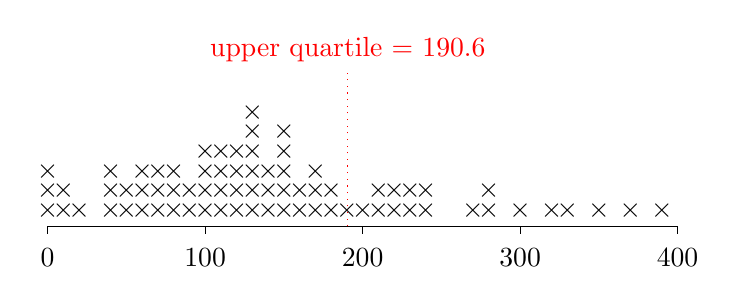
\begin{tikzpicture}
		\node at (0.00,0.25) (1) {$\times$};
		\node at (0.00,0.50) (1) {$\times$};
		\node at (0.00,0.75) (1) {$\times$};
		\node at (0.20,0.25) (1) {$\times$};
		\node at (0.20,0.50) (1) {$\times$};
		\node at (0.40,0.25) (1) {$\times$};
		\node at (0.80,0.25) (1) {$\times$};
		\node at (0.80,0.50) (1) {$\times$};
		\node at (0.80,0.75) (1) {$\times$};
		\node at (1.00,0.25) (1) {$\times$};
		\node at (1.00,0.50) (1) {$\times$};
		\node at (1.20,0.25) (1) {$\times$};
		\node at (1.20,0.50) (1) {$\times$};
		\node at (1.20,0.75) (1) {$\times$};
		\node at (1.40,0.25) (1) {$\times$};
		\node at (1.40,0.50) (1) {$\times$};
		\node at (1.40,0.75) (1) {$\times$};
		\node at (1.60,0.25) (1) {$\times$};
		\node at (1.60,0.50) (1) {$\times$};
		\node at (1.60,0.75) (1) {$\times$};
		\node at (1.80,0.25) (1) {$\times$};
		\node at (1.80,0.50) (1) {$\times$};
		\node at (2.00,0.25) (1) {$\times$};
		\node at (2.00,0.50) (1) {$\times$};
		\node at (2.00,0.75) (1) {$\times$};
		\node at (2.00,1.00) (1) {$\times$};
		\node at (2.20,0.25) (1) {$\times$};
		\node at (2.20,0.50) (1) {$\times$};
		\node at (2.20,0.75) (1) {$\times$};
		\node at (2.20,1.00) (1) {$\times$};
		\node at (2.40,0.25) (1) {$\times$};
		\node at (2.40,0.50) (1) {$\times$};
		\node at (2.40,0.75) (1) {$\times$};
		\node at (2.40,1.00) (1) {$\times$};
		\node at (2.60,0.25) (1) {$\times$};
		\node at (2.60,0.50) (1) {$\times$};
		\node at (2.60,0.75) (1) {$\times$};
		\node at (2.60,1.00) (1) {$\times$};
		\node at (2.60,1.25) (1) {$\times$};
		\node at (2.60,1.50) (1) {$\times$};
		\node at (2.80,0.25) (1) {$\times$};
		\node at (2.80,0.50) (1) {$\times$};
		\node at (2.80,0.75) (1) {$\times$};
		\node at (3.00,0.25) (1) {$\times$};
		\node at (3.00,0.50) (1) {$\times$};
		\node at (3.00,0.75) (1) {$\times$};
		\node at (3.00,1.00) (1) {$\times$};
		\node at (3.00,1.25) (1) {$\times$};
		\node at (3.20,0.25) (1) {$\times$};
		\node at (3.20,0.50) (1) {$\times$};
		\node at (3.40,0.25) (1) {$\times$};
		\node at (3.40,0.50) (1) {$\times$};
		\node at (3.40,0.75) (1) {$\times$};
		\node at (3.60,0.25) (1) {$\times$};
		\node at (3.60,0.50) (1) {$\times$};
		\node at (3.80,0.25) (1) {$\times$};
		\node at (4.00,0.25) (1) {$\times$};
		\node at (4.20,0.25) (1) {$\times$};
		\node at (4.20,0.50) (1) {$\times$};
		\node at (4.40,0.25) (1) {$\times$};
		\node at (4.40,0.50) (1) {$\times$};
		\node at (4.60,0.25) (1) {$\times$};
		\node at (4.60,0.50) (1) {$\times$};
		\node at (4.80,0.25) (1) {$\times$};
		\node at (4.80,0.50) (1) {$\times$};
		\node at (5.40,0.25) (1) {$\times$};
		\node at (5.60,0.25) (1) {$\times$};
		\node at (5.60,0.50) (1) {$\times$};
		\node at (6.00,0.25) (1) {$\times$};
		\node at (6.40,0.25) (1) {$\times$};
		\node at (6.60,0.25) (1) {$\times$};
		\node at (7.00,0.25) (1) {$\times$};
		\node at (7.40,0.25) (1) {$\times$};
		\node at (7.80,0.25) (1) {$\times$};
		
		\draw (0,0.05) -- (8,0.05);
		\draw (0,0.05) -- (0,-0.05);
		\draw (2,0.05) -- (2,-0.05);
		\draw (4,0.05) -- (4,-0.05);
		\draw (6,0.05) -- (6,-0.05);
		\draw (8,0.05) -- (8,-0.05);
		
		\node at (0,-0.35) (0) {0};
		\node at (2,-0.35) (0) {100};
		\node at (4,-0.35) (0) {200};
		\node at (6,-0.35) (0) {300};
		\node at (8,-0.35) (0) {400};
		
		\draw[red,dotted] (3.812,0.05) -- (3.812,2);
		\node[red] at (3.812,2.3) (up) {upper quartile = 190.6};
	\end{tikzpicture}
\end{center}
	
	If a normal distribution does not seem a reasonable model, an alternative is to treat the actual sample as the "population" for the simulation and take random samples with replacement from this sample. Such samples are called \begriff{bootstrap samples}. A simulation with these bootstrap samples can again show the error distribution and provide approximate values for the bias and standard error.
	
	\begin{center}
	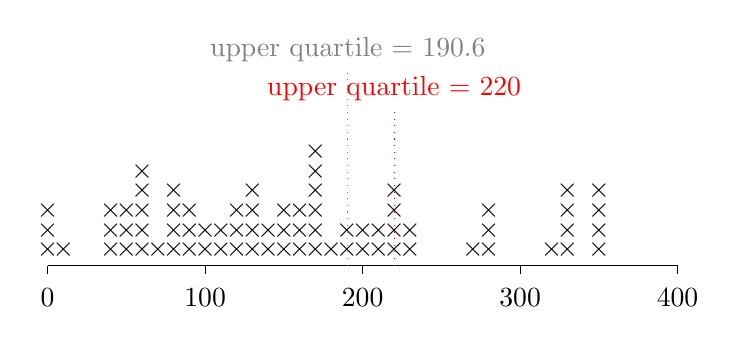
\begin{tikzpicture}
		\node at (0.00,0.25) (1) {$\times$};
		\node at (0.00,0.50) (1) {$\times$};
		\node at (0.00,0.75) (1) {$\times$};
		\node at (0.20,0.25) (1) {$\times$};
		\node at (0.80,0.25) (1) {$\times$};
		\node at (0.80,0.50) (1) {$\times$};
		\node at (0.80,0.75) (1) {$\times$};
		\node at (1.00,0.25) (1) {$\times$};
		\node at (1.00,0.50) (1) {$\times$};
		\node at (1.00,0.75) (1) {$\times$};
		\node at (1.20,0.25) (1) {$\times$};
		\node at (1.20,0.50) (1) {$\times$};
		\node at (1.20,0.75) (1) {$\times$};
		\node at (1.20,1.00) (1) {$\times$};
		\node at (1.20,1.25) (1) {$\times$};
		\node at (1.40,0.25) (1) {$\times$};
		\node at (1.60,0.25) (1) {$\times$};
		\node at (1.60,0.50) (1) {$\times$};
		\node at (1.60,0.75) (1) {$\times$};
		\node at (1.60,1.00) (1) {$\times$};
		\node at (1.80,0.25) (1) {$\times$};
		\node at (1.80,0.50) (1) {$\times$};
		\node at (1.80,0.75) (1) {$\times$};
		\node at (2.00,0.25) (1) {$\times$};
		\node at (2.00,0.50) (1) {$\times$};
		\node at (2.20,0.25) (1) {$\times$};
		\node at (2.20,0.50) (1) {$\times$};
		\node at (2.40,0.25) (1) {$\times$};
		\node at (2.40,0.50) (1) {$\times$};
		\node at (2.40,0.75) (1) {$\times$};
		\node at (2.60,0.25) (1) {$\times$};
		\node at (2.60,0.50) (1) {$\times$};
		\node at (2.60,0.75) (1) {$\times$};
		\node at (2.60,1.00) (1) {$\times$};
		\node at (2.80,0.25) (1) {$\times$};
		\node at (2.80,0.50) (1) {$\times$};
		\node at (3.00,0.25) (1) {$\times$};
		\node at (3.00,0.50) (1) {$\times$};
		\node at (3.00,0.75) (1) {$\times$};
		\node at (3.20,0.25) (1) {$\times$};
		\node at (3.20,0.50) (1) {$\times$};
		\node at (3.20,0.75) (1) {$\times$};
		\node at (3.40,0.25) (1) {$\times$};
		\node at (3.40,0.50) (1) {$\times$};
		\node at (3.40,0.75) (1) {$\times$};
		\node at (3.40,1.00) (1) {$\times$};
		\node at (3.40,1.25) (1) {$\times$};
		\node at (3.40,1.50) (1) {$\times$};
		\node at (3.60,0.25) (1) {$\times$};
		\node at (3.80,0.25) (1) {$\times$};
		\node at (3.80,0.50) (1) {$\times$};
		\node at (4.00,0.25) (1) {$\times$};
		\node at (4.00,0.50) (1) {$\times$};
		\node at (4.20,0.25) (1) {$\times$};
		\node at (4.20,0.50) (1) {$\times$};
		\node at (4.40,0.25) (1) {$\times$};
		\node at (4.40,0.50) (1) {$\times$};
		\node at (4.40,0.75) (1) {$\times$};
		\node at (4.40,1.00) (1) {$\times$};
		\node at (4.60,0.25) (1) {$\times$};
		\node at (4.60,0.50) (1) {$\times$};
		\node at (5.40,0.25) (1) {$\times$};
		\node at (5.60,0.25) (1) {$\times$};
		\node at (5.60,0.50) (1) {$\times$};
		\node at (5.60,0.75) (1) {$\times$};
		\node at (6.40,0.25) (1) {$\times$};
		\node at (6.60,0.25) (1) {$\times$};
		\node at (6.60,0.50) (1) {$\times$};
		\node at (6.60,0.75) (1) {$\times$};
		\node at (6.60,1.00) (1) {$\times$};
		\node at (7.00,0.25) (1) {$\times$};
		\node at (7.00,0.50) (1) {$\times$};
		\node at (7.00,0.75) (1) {$\times$};
		\node at (7.00,1.00) (1) {$\times$};
		
		\draw (0,0.05) -- (8,0.05);
		\draw (0,0.05) -- (0,-0.05);
		\draw (2,0.05) -- (2,-0.05);
		\draw (4,0.05) -- (4,-0.05);
		\draw (6,0.05) -- (6,-0.05);
		\draw (8,0.05) -- (8,-0.05);
		
		\node at (0,-0.35) (0) {0};
		\node at (2,-0.35) (0) {100};
		\node at (4,-0.35) (0) {200};
		\node at (6,-0.35) (0) {300};
		\node at (8,-0.35) (0) {400};
		
		\draw[gray,dotted] (3.812,0.05) -- (3.812,2.5);
		\node[gray] at (3.812,2.8) (up) {upper quartile = 190.6};
		\draw[red,dotted] (4.4,0.05) -- (4.4,2);
		\node[red] at (4.4,2.3) (up) {upper quartile = 220};
	\end{tikzpicture}
\end{center}
	\begin{center}
	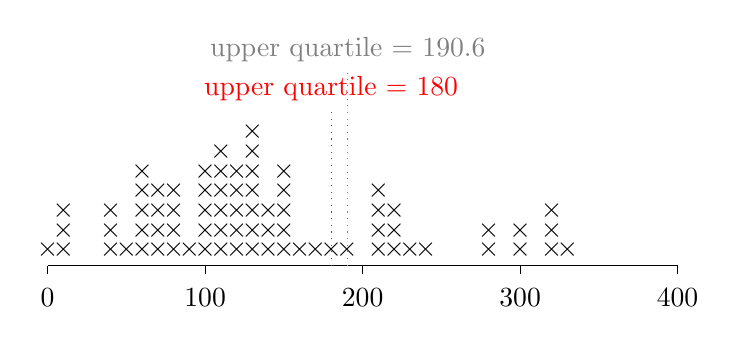
\begin{tikzpicture}
		\node at (0.00,0.25) (1) {$\times$};
		\node at (0.20,0.25) (1) {$\times$};
		\node at (0.20,0.50) (1) {$\times$};
		\node at (0.20,0.75) (1) {$\times$};
		\node at (0.80,0.25) (1) {$\times$};
		\node at (0.80,0.50) (1) {$\times$};
		\node at (0.80,0.75) (1) {$\times$};
		\node at (1.00,0.25) (1) {$\times$};
		\node at (1.20,0.25) (1) {$\times$};
		\node at (1.20,0.50) (1) {$\times$};
		\node at (1.20,0.75) (1) {$\times$};
		\node at (1.20,1.00) (1) {$\times$};
		\node at (1.20,1.25) (1) {$\times$};
		\node at (1.40,0.25) (1) {$\times$};
		\node at (1.40,0.50) (1) {$\times$};
		\node at (1.40,0.75) (1) {$\times$};
		\node at (1.40,1.00) (1) {$\times$};
		\node at (1.60,0.25) (1) {$\times$};
		\node at (1.60,0.50) (1) {$\times$};
		\node at (1.60,0.75) (1) {$\times$};
		\node at (1.60,1.00) (1) {$\times$};
		\node at (1.80,0.25) (1) {$\times$};
		\node at (2.00,0.25) (1) {$\times$};
		\node at (2.00,0.50) (1) {$\times$};
		\node at (2.00,0.75) (1) {$\times$};
		\node at (2.00,1.00) (1) {$\times$};
		\node at (2.00,1.25) (1) {$\times$};
		\node at (2.20,0.25) (1) {$\times$};
		\node at (2.20,0.50) (1) {$\times$};
		\node at (2.20,0.75) (1) {$\times$};
		\node at (2.20,1.00) (1) {$\times$};
		\node at (2.20,1.25) (1) {$\times$};
		\node at (2.20,1.50) (1) {$\times$};
		\node at (2.40,0.25) (1) {$\times$};
		\node at (2.40,0.50) (1) {$\times$};
		\node at (2.40,0.75) (1) {$\times$};
		\node at (2.40,1.00) (1) {$\times$};
		\node at (2.40,1.25) (1) {$\times$};
		\node at (2.60,0.25) (1) {$\times$};
		\node at (2.60,0.50) (1) {$\times$};
		\node at (2.60,0.75) (1) {$\times$};
		\node at (2.60,1.00) (1) {$\times$};
		\node at (2.60,1.25) (1) {$\times$};
		\node at (2.60,1.50) (1) {$\times$};
		\node at (2.60,1.75) (1) {$\times$};
		\node at (2.80,0.25) (1) {$\times$};
		\node at (2.80,0.50) (1) {$\times$};
		\node at (2.80,0.75) (1) {$\times$};
		\node at (3.00,0.25) (1) {$\times$};
		\node at (3.00,0.50) (1) {$\times$};
		\node at (3.00,0.75) (1) {$\times$};
		\node at (3.00,1.00) (1) {$\times$};
		\node at (3.00,1.25) (1) {$\times$};
		\node at (3.20,0.25) (1) {$\times$};
		\node at (3.40,0.25) (1) {$\times$};
		\node at (3.60,0.25) (1) {$\times$};
		\node at (3.80,0.25) (1) {$\times$};
		\node at (4.20,0.25) (1) {$\times$};
		\node at (4.20,0.50) (1) {$\times$};
		\node at (4.20,0.75) (1) {$\times$};
		\node at (4.20,1.00) (1) {$\times$};
		\node at (4.40,0.25) (1) {$\times$};
		\node at (4.40,0.50) (1) {$\times$};
		\node at (4.40,0.75) (1) {$\times$};
		\node at (4.60,0.25) (1) {$\times$};
		\node at (4.80,0.25) (1) {$\times$};
		\node at (5.60,0.25) (1) {$\times$};
		\node at (5.60,0.50) (1) {$\times$};
		\node at (6.00,0.25) (1) {$\times$};
		\node at (6.00,0.50) (1) {$\times$};
		\node at (6.40,0.25) (1) {$\times$};
		\node at (6.40,0.50) (1) {$\times$};
		\node at (6.40,0.75) (1) {$\times$};
		\node at (6.60,0.25) (1) {$\times$};
		
		\draw (0,0.05) -- (8,0.05);
		\draw (0,0.05) -- (0,-0.05);
		\draw (2,0.05) -- (2,-0.05);
		\draw (4,0.05) -- (4,-0.05);
		\draw (6,0.05) -- (6,-0.05);
		\draw (8,0.05) -- (8,-0.05);
		
		\node at (0,-0.35) (0) {0};
		\node at (2,-0.35) (0) {100};
		\node at (4,-0.35) (0) {200};
		\node at (6,-0.35) (0) {300};
		\node at (8,-0.35) (0) {400};
		
		\draw[gray,dotted] (3.812,0.05) -- (3.812,2.5);
		\node[gray] at (3.812,2.8) (up) {upper quartile = 190.6};
		\draw[red,dotted] (3.6,0.05) -- (3.6,2);
		\node[red] at (3.6,2.3) (up) {upper quartile = 180};
	\end{tikzpicture}
\end{center}
\end{example}

\subsection{Bootstrap distribution}

The standard error of a statistic is the standard deviation of the sample statistic. The standard error can be calculated as the standard deviation of the sampling distribution.

Bootstrap sample is a random sample taken with replacement from the original sample, of the same size as the original sample. A bootstrap statistic is the statistic computed on a bootstrap sample. A bootstrap distribution is the distribution of many bootstrap statistics. The standard error of a statistic can be estimated using the standard deviation of the bootstrap distribution.

Let $\hat{\theta}$ a statistic calculated from a sample ($\hat{\theta} = \bar{x}$). We draw $r$ observations with replacement to create a bootstrap sample and calculate the statistic $\hat{\theta}^\ast$ for this sample.
\begin{itemize}
	\item \textbf{bootstrap standard error:} the sample standard deviation of the bootstrap distribution:
	\begin{align}
		\SE_b = \sqrt{\frac{\sum (\hat{\theta}^\ast_b - \bar{\theta}^\ast)^2}{B-1}} \notag
	\end{align}
	where $B$ is the number of bootstrap replications (usually $B>10000$)
	\item \textbf{bootstrap bias:} $\bar{\theta}^\ast-\hat{\theta}$
	\item \textbf{bootstrap confidence intervals:} bootstrap percentile interval, t confidence interval with bootstrap standard error, bootstrap t-interval, etc.
\end{itemize}

\subsection{Bootstrap methods}

\begin{center}
	\begin{tabular}{p{3cm}|p{2cm}|p{2cm}|p{3cm}|p{3.5cm}}
		\textbf{Name} & \textbf{calculate} & \textbf{repeat} & \textbf{get distribution} & \textbf{confidence interval} \\
		\hline
		Bootstrap percentile CI or \person{Efron} method & $\hat{\theta}^\ast_b$ & $B$ times & $\left\lbrace \hat{\theta}^\ast_b\right\rbrace^B_{b=1}$ & $[q_{\nicefrac{\alpha}{2}},q_{1-\nicefrac{\alpha}{2}}]$ \\
		\hline
		Bootstrap CI - bootstrap t & $\frac{\hat{\theta}^\ast_b-\hat{\theta}}{\SE(\hat{\theta}^\ast_b)}$ & $B$ times & $\left\lbrace\frac{\hat{\theta}^\ast_b-\hat{\theta}}{\SE(\hat{\theta}^\ast_b)} \right\rbrace^B_{b=1}$ & $[\hat{\theta}-\SE(\hat{\theta})\cdot q_{1-\nicefrac{\alpha}{2}},\hat{\theta}-\SE(\hat{\theta})\cdot q_{\nicefrac{\alpha}{2}}]$ \\
		\hline
		Bootstrap CI symmetric t-percentile & $\frac{\hat{\theta}^\ast_b-\hat{\theta}}{\SE(\hat{\theta}^\ast_b)}$ & $B$ times & $\left\lbrace\frac{\hat{\theta}^\ast_b-\hat{\theta}}{\SE(\hat{\theta}^\ast_b)} \right\rbrace^B_{b=1}$ & $[\hat{\theta}-\SE(\hat{\theta})\cdot q_{1-\alpha},\hat{\theta}+\SE(\hat{\theta})\cdot q_{1-\alpha}]$ \\
		\hline
		Bootstrap CI \person{Hall} method & $\hat{\theta}^\ast_b-\hat{\theta}$ & $B$ times & $\left\lbrace \hat{\theta}^\ast_b - \hat{\theta} \right\rbrace^B_{b=1}$ & $[\hat{\theta}-q_{1-\nicefrac{\alpha}{2}},\hat{\theta} - q_{\nicefrac{\alpha}{2}}]$ \\
	\end{tabular}
\end{center}

\textbf{Bootstrap using t CI - \textcolor{red}{not recommended}}
\begin{align}
	\hat{\theta}\pm t_{\nicefrac{\alpha}{2}}\cdot\SE_b\notag
\end{align}
Bootstrap standard error is the sample standard deviation of the bootstrap distribution
\begin{align}
	\SE_b = \sqrt{\frac{\sum (\hat{\theta}^\ast_b - \bar{\theta}^\ast)^2}{B-1}} \notag
\end{align}
where $B$ is the number of bootstrap replications (usually $B>10000$). The bootstrap bias is $\bar{\theta}^\ast-\hat{\theta}$. It can be useful when the standard error is difficult to derive. \textcolor{red}{It has a poor performance when distributions are highly skewed.}

\textbf{Bootstrap percentile CI or \person{Elfron} method} \\
For a 90\% confidence interval keep the middle 90\%, leaving 5\% in each tail and 5\% in the head. The 90\% confidence interval boundaries would be the 5th percentile and the 95th percentile. In case we have 10000 bootstrap replications: $\theta^\ast_1\le\theta^\ast_2\le\dots\le\theta^\ast_{10000}$ the 90\% confidence interval is $[\theta^\ast_{500},\theta^\ast_{9500}]$.
\begin{itemize}
	\item \textbf{Advantages:} A very intuitive and easy to implement method. Can also outperform some other bootstrap CI methods for skewed distributions.
	\item \textbf{Disadvantages:} Can be too narrow for small samples.
\end{itemize}